% =============================================================================
% CHAPITRE 2 — PRISE EN MAIN ET CONCEPTION DE LA SOLUTION
% =============================================================================

\chapter{Prise en main et conception de la solution}
\label{chap:prise_en_main_conception}

% =============================================================================
% 2.1 DÉCOUVERTE DE L'ENVIRONNEMENT ISOGEO
% =============================================================================

\section{Découverte de l'environnement Isogeo}
\label{sec:decouverte_environnement_isogeo}

% -----------------------------------------------------------------------------
% 2.1.1 Formation aux solutions existantes
% -----------------------------------------------------------------------------

\subsection{Formation aux solutions existantes}
\label{subsec:formation_solutions_existantes}

Les premières semaines ont été consacrées à la découverte des solutions
développées par Isogeo. Cette phase correspondait à la période d'intégration.
Elle devait me permettre de comprendre l'entreprise, son organisation et le
rôle de Scan dans l'ensemble de l'écosystème.

Au cours de cette période, j'ai regardé plusieurs webinaires de présentation de
la solution. J'ai également lu des documents liés à l'entreprise, aux produits
Isogeo et aux pratiques de développement mises en place au sein de l'équipe
Produit.

Cette étape était importante pour mieux situer la mission dans le fonctionnement
réel du produit.

Les formations ont porté sur les principaux services utilisés par les clients.
L'\textit{App} constitue l'espace de travail principal pour gérer les catalogues
et documenter les fiches de métadonnées. \textit{Manage} est destiné à
l'administration des groupes, des utilisateurs et des applications associées.
\textit{OpenCatalog} et le \textit{Portail de données} servent à publier et à
valoriser les catalogues auprès des utilisateurs finaux.

D'autres outils complètent cet ensemble. L'\textit{Extracteur} permet de rendre
les données plus facilement téléchargeables. Les plugins QGIS et ArcGIS Pro
facilitent l'accès aux données depuis les logiciels SIG utilisés au quotidien
par les géomaticiens.

Cette découverte m'a permis de comprendre que Scan n'est pas un composant isolé.
Il intervient en amont du catalogue. Son rôle est de recenser les ressources
disponibles, d'en extraire les informations techniques utiles et de préparer la
mise à jour des fiches de métadonnées.

% Image à inclure :
% Une vue synthétique de l'écosystème Isogeo montrant le lien entre Scan,
% l'App, Manage, OpenCatalog, le Portail de données, l'Extracteur et les plugins.

% -----------------------------------------------------------------------------
% 2.1.2 Prise en main du produit Scan
% -----------------------------------------------------------------------------

\subsection{Prise en main du produit Scan}
\label{subsec:prise_en_main_scan}

La prise en main de Scan a ensuite permis d'identifier les principales étapes
réalisées par le produit. Les traitements reposent sur trois opérations
centrales : le listing, la signature et la documentation des données.

Le listing sert à inventorier les ressources accessibles dans une source. La
signature permet de détecter si une ressource a changé depuis une exécution
précédente. La documentation produit les informations techniques nécessaires à
la création ou à la mise à jour d'une fiche de métadonnées.

Cette phase a aussi permis de comprendre les contraintes du produit. Le logiciel doit
fonctionner chez les clients, dans des environnements différents, avec des
sources de données variées. Les traitements doivent donc être fiables,
prévisibles et compatibles avec le fonctionnement existant.

La prise en main ne s'est pas limitée à une lecture théorique. Elle s'est faite
progressivement, en échangeant avec l'équipe, en observant le comportement du
produit et en réalisant des premiers tests sur des sources simples.

% Image à inclure :
% Un schéma simple du fonctionnement de Scan : source de données, listing,
% signature, documentation, puis mise à jour du catalogue.

% =============================================================================
% 2.2 ANALYSE ET DOCUMENTATION DE L'EXISTANT
% =============================================================================

\section{Analyse et documentation de l'existant}
\label{sec:analyse_documentation_existant}

% -----------------------------------------------------------------------------
% 2.2.1 Étude du code Python existant
% -----------------------------------------------------------------------------

\subsection{Étude du code Python existant}
\label{subsec:etude_code_python_existant}

Avant mon arrivée, une partie de la migration avait déjà été engagée. Il
existait donc du code Python à lire, à comprendre et à replacer dans
l'architecture générale de Scan.

Cette étape a consisté à parcourir les modules existants, à identifier les
classes principales et à comprendre la manière dont les traitements étaient
organisés. L'objectif était de repérer les éléments déjà réutilisables et les choix de conception à conserver pour la suite
du développement.

L'analyse du code a aussi permis de mieux comprendre les responsabilités de
chaque module. Certains éléments étaient communs à plusieurs sources, comme la
gestion des paramètres, la structure des résultats ou le traitement des erreurs.
D'autres dépendaient directement du type de source analysée.

Cette lecture progressive a servi de base au travail de développement. Elle a
évité de repartir de zéro et a permis de rester cohérent avec les choix déjà
faits par l'équipe.

% -----------------------------------------------------------------------------
% 2.2.2 Documentation de l'existant
% -----------------------------------------------------------------------------

\subsection{Documentation de l'existant}
\label{subsec:documentation_existant}

La documentation a accompagné cette phase d'analyse. Elle avait pour but de
conserver les informations utiles à la poursuite de la migration et de rendre
plus lisible le fonctionnement du code existant.

Il s'agissait principalement d'une documentation directement liée au code
source. Les classes et les fonctions étaient décrites à l'aide de commentaires
de documentation, placés sous leur définition. Ces descriptions précisaient le
rôle du traitement, les paramètres attendus, les valeurs retournées et les cas
particuliers à connaître.

Cette documentation était utile pendant la prise en main, mais aussi pour toute
personne devant éventuellement reprendre le code source. Elle facilitait les
échanges techniques et permettait de partager plus facilement ce qui avait été
compris ou vérifié.

\begin{figure}[H]
\centering
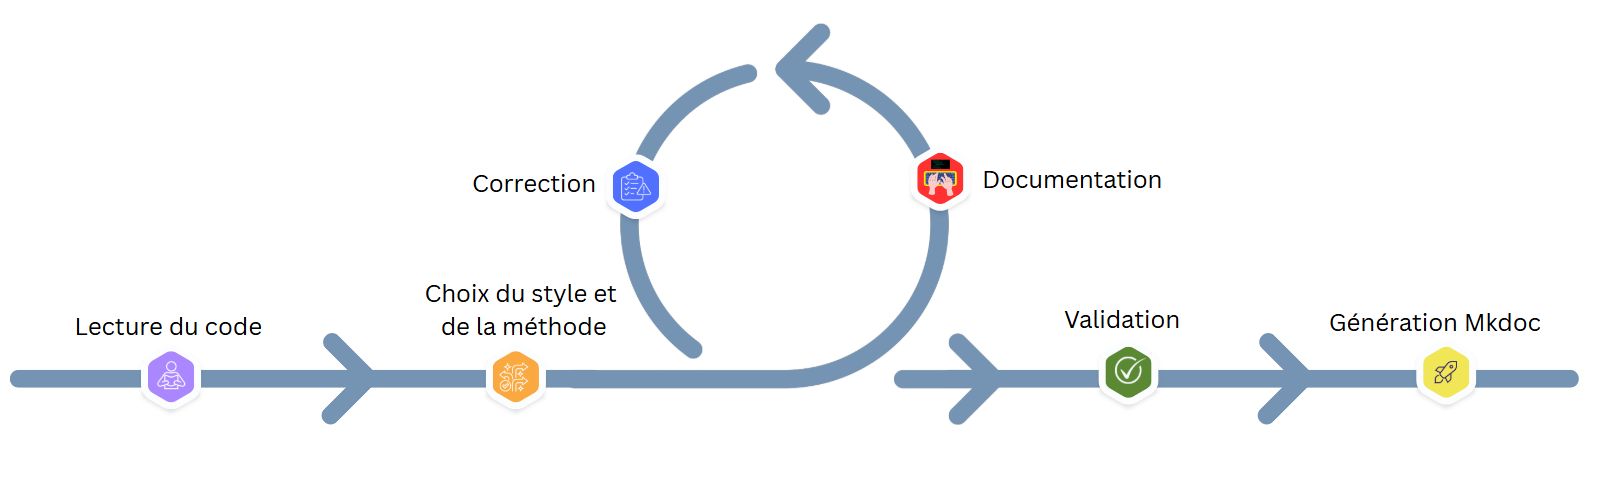
\includegraphics[width=\textwidth]{figures/isogeo/process_doc.png}
\caption{Processus de documentation du code source}
\label{fig:processus_documentation_code}
\end{figure}

Afin de rendre cette documentation plus accessible, nous avons également produit
un site statique avec \textit{MkDocs} et \textit{mkdocstrings}. Cet outil permet
de générer automatiquement des pages de documentation à partir des informations
présentes dans le code. Le résultat est plus simple à consulter qu'une lecture
directe des fichiers Python.

\begin{figure}[H]
\centering
\begin{subfigure}[t]{0.48\textwidth}
\centering
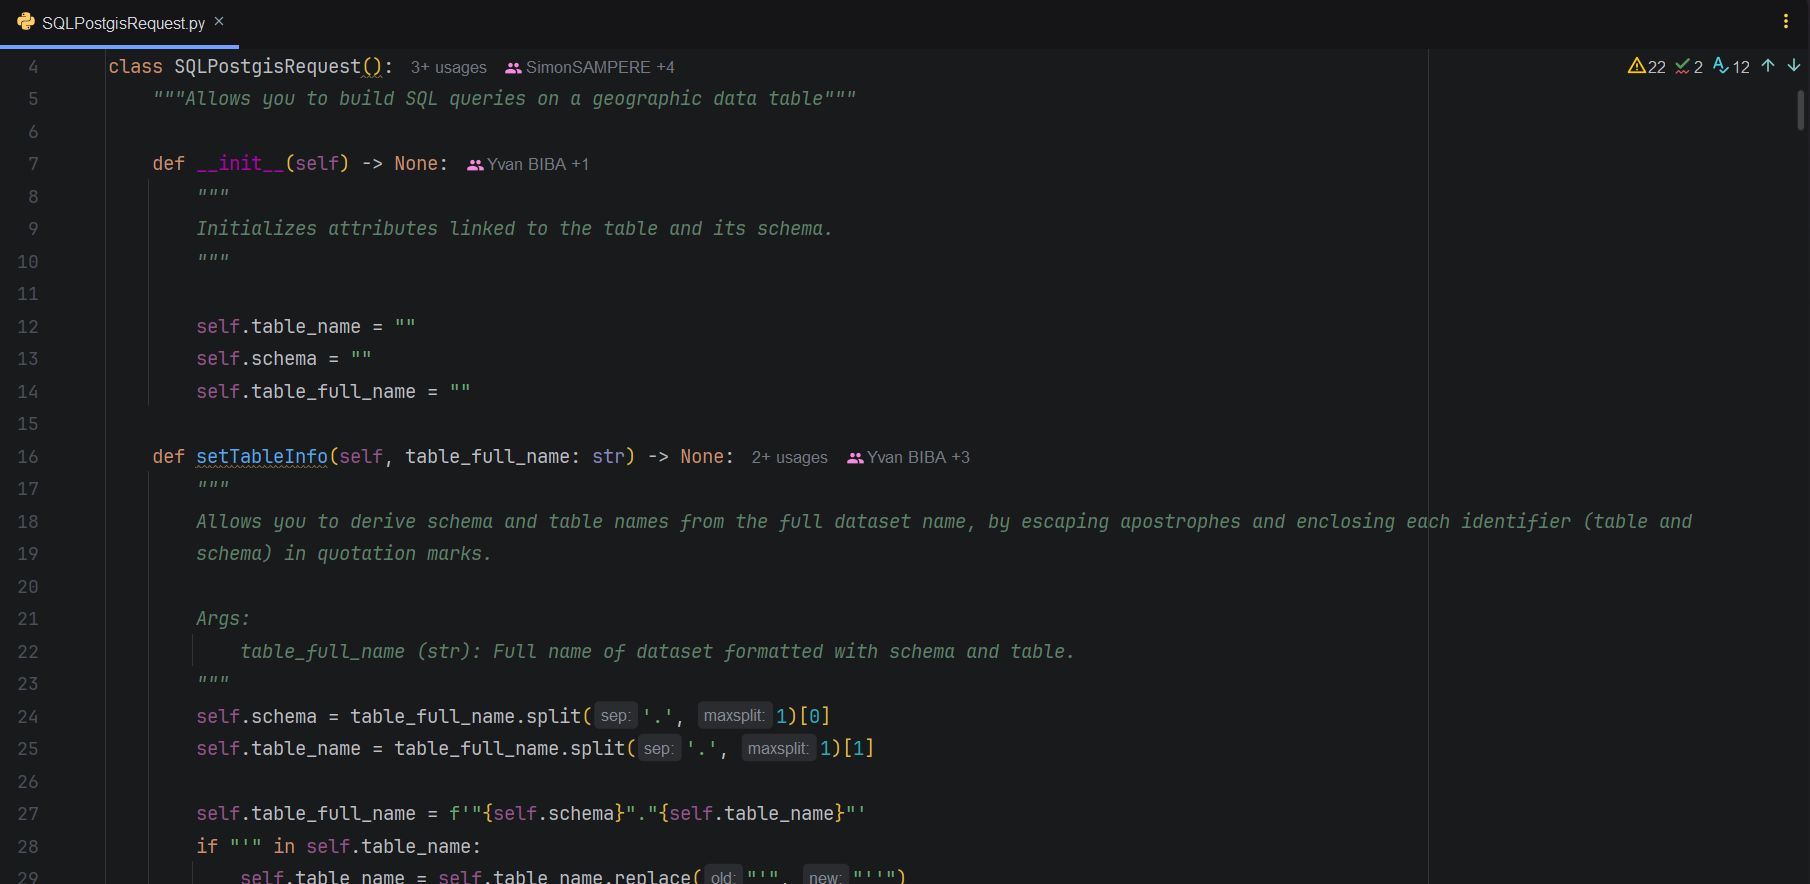
\includegraphics[width=\textwidth]{figures/isogeo/raw_doc.png}
\caption{Documentation dans le code source}
\label{fig:documentation_code_brut}
\end{subfigure}
\hfill
\begin{subfigure}[t]{0.48\textwidth}
\centering
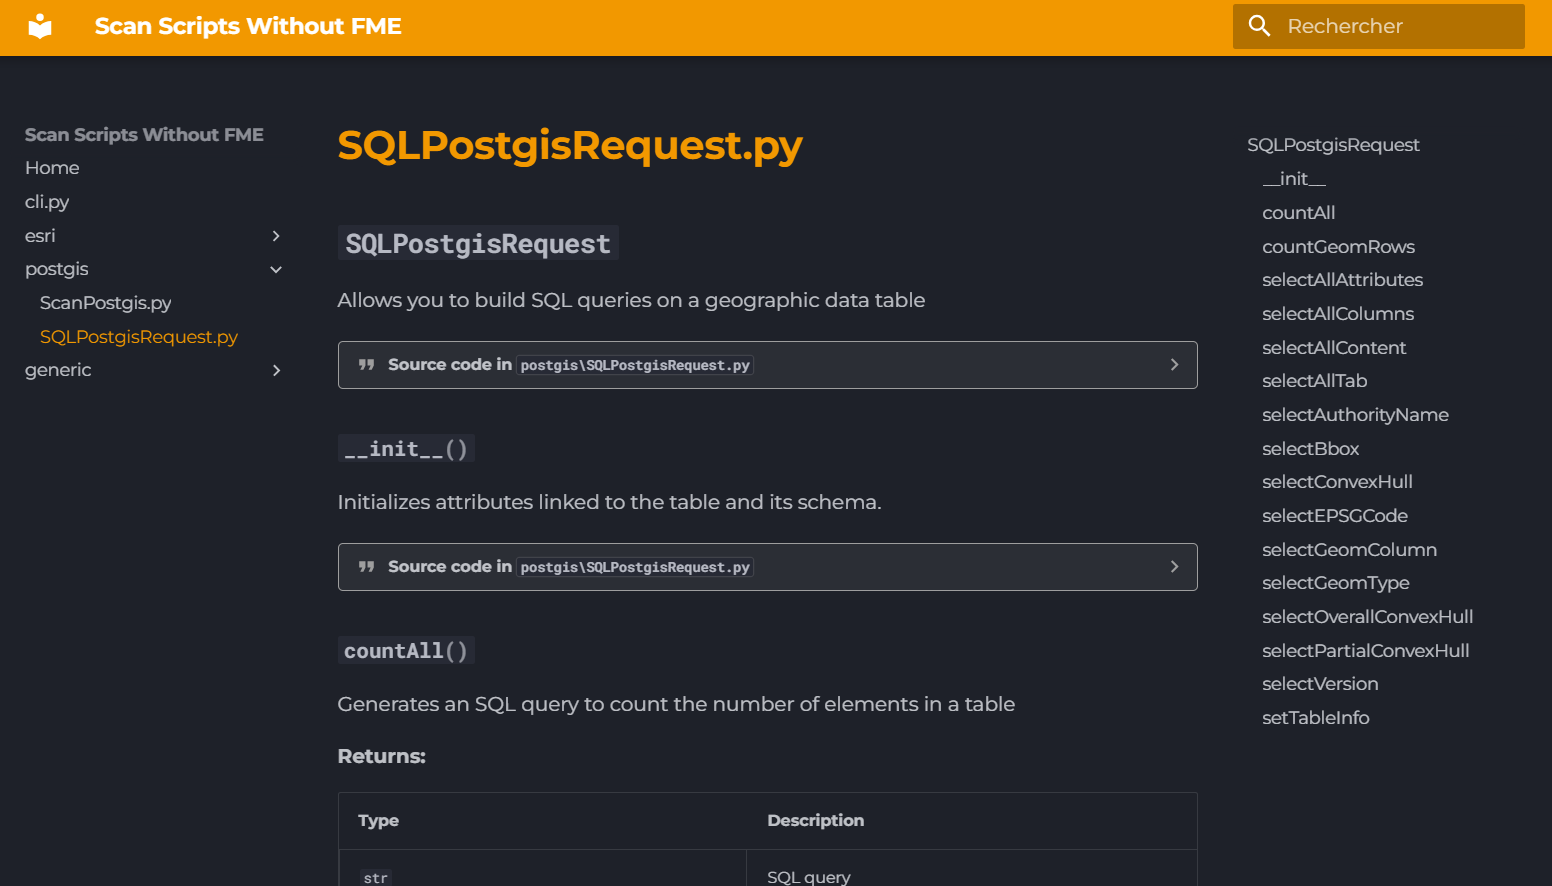
\includegraphics[width=\textwidth]{figures/isogeo/static_site.png}
\caption{Site statique généré}
\label{fig:documentation_site_statique}
\end{subfigure}
\caption{Passage du code brut au site statique de documentation}
\label{fig:site_statique_documentation}
\end{figure}


% =============================================================================
% 2.3 EXPÉRIMENTATIONS AVEC GDAL ET OGR
% =============================================================================

\section{Expérimentations avec GDAL et OGR}
\label{sec:experimentations_gdal_ogr}

% -----------------------------------------------------------------------------
% 2.3.1 Prise en main des bibliothèques
% -----------------------------------------------------------------------------

\subsection{Prise en main des bibliothèques}
\label{subsec:prise_en_main_gdal_ogr}

GDAL et OGR sont des bibliothèques largement utilisées pour lire, manipuler et
analyser des données géographiques. Dans le cadre de la mission, elles
représentaient une solution importante pour remplacer une partie des traitements
historiquement réalisés avec FME.

La prise en main a d'abord porté sur la lecture de fichiers vectoriels et
raster. Il s'agissait de vérifier comment accéder aux couches, aux champs, au
système de coordonnées, à l'emprise ou encore au nombre d'entités.

Ces premiers essais ont permis de mieux comprendre la manière dont GDAL et OGR
présentent les données. Ils ont aussi montré que les informations disponibles
peuvent varier selon les formats, les pilotes utilisés et la qualité des données
en entrée.

% -----------------------------------------------------------------------------
% 2.3.2 Réalisation de tests techniques
% -----------------------------------------------------------------------------

\subsection{Réalisation de tests techniques}
\label{subsec:tests_techniques_gdal_ogr}

Des tests techniques ont ensuite été réalisés sur les formats rasters et vecteurs.
L'objectif était de vérifier ce que les bibliothèques permettaient d'obtenir et
de repérer les comportements particuliers dès le début du travail.

Ces tests ont porté sur des opérations simples, comme l'ouverture d'une source,
la lecture des couches, la récupération des champs ou l'accès aux informations
géographiques principales. Ils ont aussi permis d'observer les erreurs
renvoyées lorsque la donnée était absente, invalide ou mal structurée.

Cette étape a été utile pour préparer la suite du développement. Elle a permis
d'identifier les possibilités offertes par GDAL et OGR, mais aussi certaines
limites à prendre en compte dans l'architecture de la solution.

% Image à inclure :
% Un tableau ou une capture présentant quelques formats testés avec GDAL/OGR et
% les informations récupérées.

% =============================================================================
% 2.4 CONCEPTION DE LA SOLUTION
% =============================================================================

\section{Conception de la solution}
\label{sec:conception_solution}

% -----------------------------------------------------------------------------
% 2.4.1 Définition de l'architecture
% -----------------------------------------------------------------------------

\subsection{Définition de l'architecture}
\label{subsec:def_architecture}

Après la phase de prise en main, il a été nécessaire de définir une organisation
claire pour les nouveaux traitements. L'objectif était de construire une
solution capable de prendre en charge plusieurs sources, sans dupliquer
inutilement la logique commune.

L'architecture devait séparer les responsabilités. Les éléments communs
devaient gérer les paramètres d'entrée, la structure des résultats, les erreurs
et les étapes générales du traitement. Les éléments propres à chaque source
devaient se concentrer sur les particularités du format ou de la technologie
utilisée.

Cette organisation permettait de faciliter les évolutions futures. Lorsqu'une
nouvelle source devait être prise en charge, l'idée était de pouvoir réutiliser
le socle commun et d'ajouter uniquement les traitements spécifiques nécessaires.

La conception devait aussi tenir compte de l'intégration dans Scan. Les scripts
ne devaient pas seulement fonctionner seuls. Ils devaient produire des résultats
exploitables par le reste du produit et respecter les conventions déjà en place.

% Image à inclure :
% Un schéma d'architecture montrant un socle commun et des modules spécifiques
% par source de données.

% -----------------------------------------------------------------------------
% 2.4.2 Définition de la méthode de validation
% -----------------------------------------------------------------------------

\subsection{Définition de la méthode de validation}
\label{subsec:def_methode_validation}

La méthode de validation dépendait du type de traitement étudié. Pour l'inventaire des données et la documentation, elle reposait principalement sur des tests de
non-régression. L'objectif était de comparer les sorties produites par les
nouveaux scripts Python avec les résultats obtenus par les workbenches FME de
référence.

Pour la documentation des données, la comparaison portait sur l'ensemble des
métadonnées produites : nom de la ressource, système de projection, emprise,
enveloppe convexe, champs, types de géométrie et autres informations attendues
par Scan.

Pour la signature, la validation cherchait surtout à vérifier l'intégrité du
calcul. Il fallait s'assurer que le hash restait stable lorsque la donnée ne
changeait pas, mais qu'il évoluait lorsqu'une modification réelle était
effectuée.

\begin{table}[H]
\centering
\begin{tabularx}{\textwidth}{>{\bfseries}p{2.7cm}XX}
\toprule
Type de test & Objectif & Application \\
\midrule
Non-régression & Comparer les sorties Python avec les résultats FME de
référence. & Inventaire et documentation. \\
Intégrité de la signature & Vérifier que le hash réagit correctement aux
modifications de la donnée. & Signature. \\
Performance & Mesurer le comportement des scripts sur des volumes de données
importants. & Inventaire, documentation et signature. \\
\bottomrule
\end{tabularx}
\caption{Principaux tests prévus pour valider les traitements Python}
\label{tab:tests_validation_python}
\end{table}

\textbf{NB :} les tests d'intégrité de la signature regroupaient plusieurs
vérifications. La \textbf{constance} permettait de vérifier qu'une même donnée
produisait la même signature entre deux exécutions. Les \textbf{cas limites}
servaient à contrôler le comportement face à une table absente, une source
invalide ou des types inconnus. L'\textbf{isolation} vérifiait qu'une
modification sur une couche ne modifiait pas la signature d'une autre couche.
Les tests \textbf{spatiaux} portaient sur les modifications géométriques ou
d'emprise. Les tests \textbf{structurels} permettaient de détecter un changement
de schéma, comme l'ajout d'une colonne. Enfin, les tests de
\textbf{sensibilité} vérifiaient que toute modification significative de la
donnée était bien prise en compte dans le hash.

Ces tests permettaient d'identifier rapidement les écarts avec le comportement
historique de Scan. Lorsqu'une différence était détectée, elle était analysée
pour déterminer s'il s'agissait d'une régression, d'un cas particulier ou d'un
ajustement acceptable.

% =============================================================================
% 2.5 PRÉPARATION DU PACKAGING
% =============================================================================

\section{Préparation du packaging}
\label{sec:preparation_packaging}

% -----------------------------------------------------------------------------
% 2.5.1 Objectifs du packaging
% -----------------------------------------------------------------------------

\subsection{Objectifs du packaging}
\label{subsec:objectifs_packaging}

Un autre enjeu important concernait la distribution des traitements Python. La
solution devait pouvoir être exécutée dans un environnement Windows sans
installation locale de Python.

Le packaging avait donc pour objectif de regrouper les scripts, les
bibliothèques nécessaires et les dépendances géospatiales dans un exécutable
autonome. Cette approche permettait de simplifier le déploiement et de limiter
les prérequis côté utilisateur.

La difficulté principale venait des bibliothèques géospatiales. GDAL et OGR
sont des outils puissants, mais leur installation peut être complexe dans un
environnement Windows classique. Ils reposent sur plusieurs dépendances natives
et leur configuration peut varier selon les versions installées.

Il était donc important de produire un exécutable qui embarque directement ces
éléments. L'objectif était d'éviter aux utilisateurs et aux développeurs de se
poser des questions sur l'installation manuelle des modules, en particulier pour
GDAL. Le processus de génération devait donc être fiable, reproductible et
maîtrisé.

% -----------------------------------------------------------------------------
% 2.5.2 Mise en place d'un environnement Docker
% -----------------------------------------------------------------------------

\subsection{Mise en place d'un environnement Docker}
\label{subsec:environnement_docker}

Pour répondre à ce besoin, la génération de l'exécutable devait être réalisée
dans un environnement Docker. L'objectif était d'avoir Docker comme seul
prérequis pour construire l'exécutable.

Cette organisation permettait de maîtriser l'environnement de construction. Les
versions de Python, de PyInstaller, de GDAL et des autres dépendances pouvaient
être fixées dans une image dédiée. La génération ne dépendait donc plus des
bibliothèques installées sur le poste du développeur.

Plusieurs approches ont été étudiées pour intégrer GDAL dans cet environnement.
Les premiers essais ont notamment porté sur les wheels Python, c'est-à-dire des
paquets déjà préparés pour faciliter l'installation des bibliothèques. Cette
solution était simple à tester, mais la source utilisée pour ces wheels n'était
pas suffisamment stable ni maintenue de façon durable. Pour une solution comme
Isogeo, qui doit rester fiable dans le temps, cette approche n'était donc pas la
plus adaptée.

Une autre piste consistait à utiliser OSGeo, une distribution Windows regroupant
plusieurs outils de géomatique, dont GDAL. Cette approche avait l'avantage
d'être proche des installations classiques du domaine. En revanche, elle
produisait un livrable beaucoup plus lourd et dépendait de chemins
d'installation susceptibles de changer selon les versions. Cela risquait de
rendre le Dockerfile plus difficile à maintenir.

L'approche Conda a finalement été retenue. Conda permet de créer un
environnement isolé avec des versions précises des outils utilisés. Cela
permettait de figer plus facilement les versions de Python, GDAL, PyInstaller et
des bibliothèques associées. Cette solution produisait également un dossier
final plus léger et un environnement plus stable.

Le processus a donc été organisé en deux étapes. Une première image Docker
servait de base et contenait l'environnement Python avec les dépendances
géospatiales principales. Une seconde image, dédiée à la construction, ajoutait
le code source de Scan, installait les dépendances propres au projet et lançait
le script de génération de l'exécutable.

Cette séparation facilitait la maintenance. L'image de base pouvait être
réutilisée tant que les versions principales ne changeaient pas. L'image de
construction pouvait ensuite être régénérée à partir du code courant.

Un point particulier concernait les données internes utilisées par GDAL,
notamment celles de la bibliothèque PROJ. Elles devaient être correctement
embarquées avec l'exécutable afin que l'application utilise les bonnes données
au moment de son exécution, sans dépendre d'une installation présente sur la
machine.

Cette étape préparait l'industrialisation de la solution. Elle devait permettre
de passer progressivement de scripts de développement à un programme Windows
généré de manière fiable, reproductible et utilisable dans le contexte réel de
Scan.

% Image à inclure :
% Un schéma simple du processus de packaging : image Docker de base, image de
% build, code source, PyInstaller, exécutable Windows.
